\documentclass[conference]{IEEEtran}
\IEEEoverridecommandlockouts
% Based on the IEEE conference template (6/27/2024).

\usepackage{cite}
\usepackage{amsmath,amssymb,amsfonts}
\usepackage{multirow}
\usepackage{graphicx}
\usepackage{textcomp}
\usepackage{xcolor}
\def\BibTeX{{\rm B\kern-.05em{\sc i\kern-.025em b}\kern-.08em
    T\kern-.1667em\lower.7ex\hbox{E}\kern-.125emX}}

% Handy shorthands
\newcommand{\Scoarse}{S_{\mathrm{coarse}}}
\newcommand{\Sfine}{S_{\mathrm{fine}}}
\newcommand{\Sfinal}{S_{\mathrm{final}}}

\begin{document}

\title{I-JEPA-AD: Decoder-Free Latent Anomaly Detection with Coarse-to-Fine Adaptive Masking}

\author{\IEEEauthorblockN{1\textsuperscript{st} Aryan Jawanjal}
\IEEEauthorblockA{\textit{Dept.\ of Computer Science and Engineering} \\
\textit{Ramdeobaba University}\\
\mbox{Nagpur, India}\\
aryanjawanjal8@gmail.com}
\and
\IEEEauthorblockN{2\textsuperscript{nd} Akshat Tiwari}
\IEEEauthorblockA{\textit{Dept.\ of Computer Science and Engineering} \\
\textit{Ramdeobaba University}\\
\mbox{Nagpur, India}\\
tiwariar\_10@rknec.edu}
\and
\IEEEauthorblockN{3\textsuperscript{rd} Arnav Milmile}
\IEEEauthorblockA{\textit{Dept.\ of Computer Science and Engineering} \\
\textit{Ramdeobaba University}\\
\mbox{Nagpur, India}\\
arnavmilmile1@gmail.com}
\and
\IEEEauthorblockN{4\textsuperscript{th} Aashutosh Dubey}
\IEEEauthorblockA{\textit{Dept.\ of Computer Science and Engineering} \\
\textit{Ramdeobaba University}\\
\mbox{Nagpur, India}\\
kailashdubey@outlook.com}
\and
\IEEEauthorblockN{Dr. Sunita G. Rawat}
\IEEEauthorblockA{\textit{Project Guide} \\
\textit{Ramdeobaba University}\\
\mbox{Nagpur, India}}
}

\maketitle

\begin{abstract}
Unsupervised visual anomaly detection for industrial inspection is dominated by pixel-reconstruction models, which need heavy decoders, and by nearest-neighbour feature banks, whose memory grows with the training set. We study a third option: a decoder-free detector that predicts masked regions entirely in the latent space of a frozen I-JEPA ViT-g/16 encoder. A small Transformer predictor is trained only on cached latents of defect-free images, and anomalies are scored by the cosine discrepancy between predicted and actual latents. A coarse-to-fine masking scheme evaluates sixteen coarse blocks first and runs single-patch fine masks only where a gate flags a suspicious region, instead of masking every patch densely. On a three-category pilot of MVTec AD (bottle, capsule, hazelnut) the adaptive pipeline reaches a mean pixel AUROC of 0.840 with about 16 masks per image, a 92 percent reduction from 196 dense masks, and end-to-end latency of 134 ms versus 350 ms for dense masking on an 8 GB RTX 4060. However, with the default gate the fine stage almost never fires. A gate calibrated on nominal validation images together with a top-5 image score lifts mean image AUROC from 0.750 to 0.796 and mean pixel AUROC to 0.850 at 35 masks per image, but the gains are statistically inconclusive in most categories and AUPRO does not improve. In this original pipeline capsule is near chance and a nearest-neighbour baseline on the same latents is clearly stronger (mean pixel AUROC 0.956). We then choose settings on synthetic defects pasted onto nominal validation images, never on the test split. Using mid-level encoder tokens (layer 32 of 40) instead of the final layer and normalising scores per token position raises mean image AUROC (top-3 score) to 0.920, mean pixel AUROC to 0.962 and mean AUPRO from 0.480 to 0.813 at the same 16 masks per image, with paired-bootstrap improvements over the original pipeline in all three categories; capsule top-3 image AUROC rises from 0.51 to 0.77. A nearest-neighbour reference on the same tokens remains stronger at image level (mean 0.97), and a re-selection of the scoring settings for layer 32 did not beat the configuration fixed beforehand. We report these results, the selection protocol that avoids test-set tuning, and the limitations of the pilot.
\end{abstract}

\begin{IEEEkeywords}
anomaly detection, I-JEPA, latent prediction, masked modeling, industrial inspection, MVTec AD
\end{IEEEkeywords}

%==============================================================================
\section{Introduction}
Automated detection and localisation of surface defects is central to industrial quality control. Because defective samples are rare and defect types are open-ended, the standard setting is unsupervised: a model is trained on defect-free (nominal) images only and must flag anything that deviates from them at test time \cite{bergmann2019mvtec,bergmann2021mvtec}.

Two families of methods dominate. Reconstruction-based approaches (autoencoders, GANs, masked autoencoders and inpainting networks) assume that anomalies cannot be reconstructed well \cite{he2022mae,zavrtanik2021inpainting,zavrtanik2021draem}. They pay for a pixel decoder, spend capacity on irrelevant high-frequency texture, and can generalise so well that they reconstruct the defect (the ``identity trap''). Embedding-based approaches such as PaDiM and PatchCore compare test patch features with those of nominal images \cite{defard2021padim,roth2022patchcore}. They are accurate, but PatchCore stores a memory bank whose size scales with the number of training patches.

The Joint-Embedding Predictive Architecture (I-JEPA) offers a different route: a model learns to predict the \emph{representations} of masked image blocks from visible context, without ever generating pixels \cite{assran2023ijepa,lecun2022path}. This suggests an anomaly detector with no decoder, in which a region is anomalous when its latent cannot be predicted from its surroundings. Two practical issues arise. First, a dense sliding-window evaluation of the predictor over every patch is redundant, since most of an industrial image is nominal. Second, the frozen ViT-g/16 backbone has about one billion parameters, so training and inference must fit a consumer GPU.

This paper reports a pilot study of \emph{I-JEPA-AD}, a decoder-free latent anomaly detector with a coarse-to-fine adaptive masking scheme designed for an 8 GB GPU. Our contributions are:
\begin{itemize}
\item A decoder-free pipeline that caches frozen I-JEPA ViT-g/16 latents offline, trains a lightweight Transformer predictor on nominal latents only, and scores anomalies by cosine discrepancy (Section~\ref{sec:method}).
\item A coarse-to-fine inference scheme with score fusion, together with predictor training masks that match the masks used at inference.
\item A validation-only protocol to calibrate the fine-stage gate and to choose a more robust top-k image score, with paired-bootstrap confidence intervals, so that no choice is tuned on the test labels (Section~\ref{sec:calib}).
\item A measured comparison against fixed-mask, dense-mask and nearest-neighbour references on MVTec AD bottle, capsule and hazelnut, including accuracy, number of predictor passes, latency and GPU memory, and an explicit account of where the approach fails (Sections~\ref{sec:results} and~\ref{sec:disc}).
\end{itemize}

%==============================================================================
\section{Related Work}
\textbf{Reconstruction-based detection.} Autoencoder, GAN and masked-autoencoder (MAE) detectors reconstruct nominal images and score by reconstruction error \cite{he2022mae,zavrtanik2021draem}. Reconstruction by inpainting reduces the identity trap by hiding regions before reconstruction \cite{zavrtanik2021inpainting}. All of these require a decoder that operates in pixel space.

\textbf{Embedding-based detection.} PaDiM models per-position Gaussian statistics of pretrained features \cite{defard2021padim}. PatchCore stores a coreset of nominal patch features and scores a test patch by its nearest-neighbour distance \cite{roth2022patchcore}. EfficientAD targets millisecond-level latency with a lightweight student-teacher design \cite{batzner2024efficientad}. Libraries such as Anomalib standardise the evaluation of these methods \cite{akcay2022anomalib}.

\textbf{Joint-embedding prediction.} I-JEPA learns by predicting target-block representations from a context block in latent space, which avoids pixel-level detail and hand-crafted augmentations \cite{assran2023ijepa}. Its use for \emph{anomaly localisation}, and in particular how to spend predictor evaluations economically, has received little study; this is the gap addressed here.

%==============================================================================
\section{Method}\label{sec:method}
Fig.~\ref{fig:arch} gives an overview. The encoder is frozen throughout; only the predictor is trained.

\begin{figure}[t]
\centering
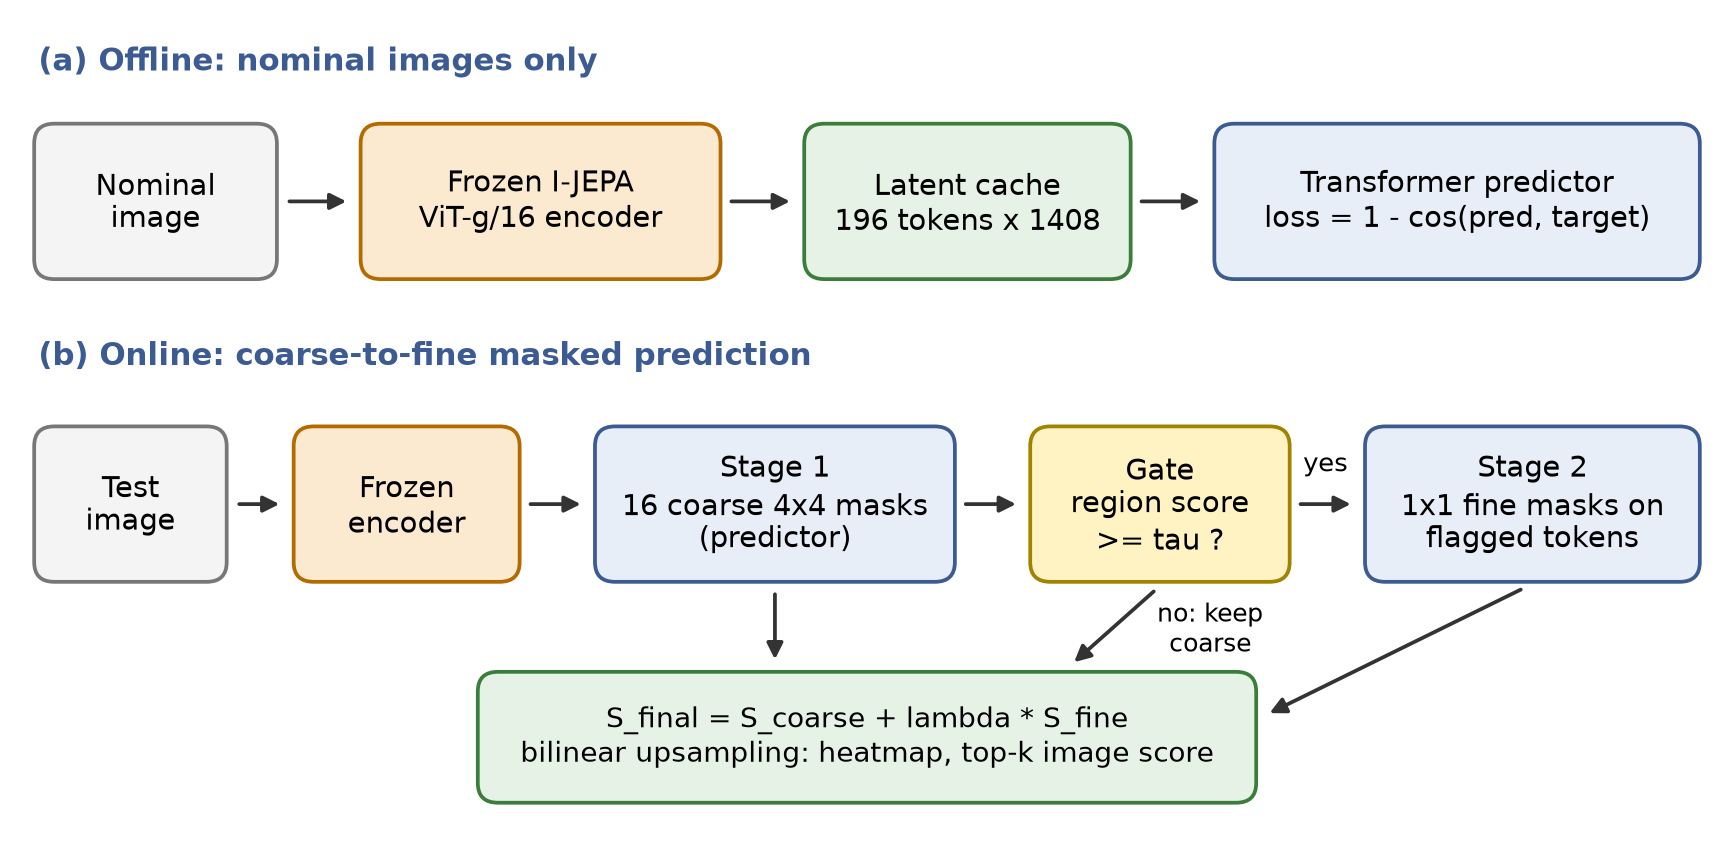
\includegraphics[width=\columnwidth]{figures/architecture.png}
\caption{I-JEPA-AD overview. (a) Latents of nominal images are cached once and used to train the predictor. (b) At test time a coarse pass is followed by a gated fine pass, and the two score maps are fused.}
\label{fig:arch}
\end{figure}

\subsection{Frozen encoder and latent cache}
An image is resized to $224\times224$ and normalised with ImageNet statistics. The official I-JEPA ViT-g/16 (ImageNet-22K) target encoder, with about $1.01\times10^{9}$ parameters, maps it to a $14\times14$ grid of 196 patch tokens $z_i\in\mathbb{R}^{1408}$. Since the encoder is frozen, every image is encoded once and the latents are stored in a cache whose identity includes the checkpoint hash, preprocessing specification and the SHA-256 of the image content. This decouples predictor training from the 16.5~GB checkpoint and keeps training within an 8~GB budget.

\subsection{Latent predictor}
The predictor receives all 196 latents together with a binary target mask $m\in\{0,1\}^{196}$. Masked tokens are replaced by a learned mask token, a learned positional embedding is added, and a Transformer encoder (hidden size 512, 4 layers, 8 heads, MLP ratio 4, about 14\,M parameters) outputs a prediction $\hat z_i\in\mathbb{R}^{1408}$ for every token after a linear projection. The model is trained on nominal images only with
\begin{equation}
\mathcal{L}=\frac{1}{|M|}\sum_{i\in M}\bigl(1-\cos(\hat z_i, z_i)\bigr),
\label{eq:loss}
\end{equation}
where $M$ is the set of masked tokens and the target $z_i$ is the cached latent. The loss is evaluated on masked tokens only, and the masked input is replaced by the mask token before any computation, so target latents cannot reach the predictor.

\textbf{Inference-aligned training masks.} Inference scores either one $4\times4$ coarse block or single tokens, so training masks follow the same geometry: with probability 0.5 a row hides one of the grid-aligned $4\times4$ coarse windows, otherwise it hides up to eight mutually non-adjacent single tokens. This replaces a random-scatter mask whose geometry differs from what is scored at test time.

\subsection{Coarse-to-fine inference}
The anomaly score of a token is the cosine discrepancy
\begin{equation}
s_i = 1-\cos(\hat z_i, z_i)\in[0,2].
\end{equation}
\textbf{Stage 1 (coarse).} The grid is partitioned into 16 non-overlapping $4\times4$ windows (narrower at the edge since $14$ is not a multiple of $4$). Each window is masked in turn, and the predictor yields $s_i$ for its tokens; this gives the coarse map $\Scoarse$ using 16 predictor passes. The region score $r_i$ of token $i$ is the mean coarse score of its window.

\textbf{Stage 2 (adaptive fine).} Every token whose region score satisfies $r_i\ge\tau$ receives its own $1\times1$ mask and an extra predictor pass; the resulting map is $\Sfine$ (zero elsewhere). If the gate never fires, the method reduces to the fixed coarse scheme; if it fires everywhere, it becomes dense masking with 196 single-token masks.

\textbf{Fusion and image score.} The final map is
\begin{equation}
\Sfinal=\Scoarse+\lambda\,\Sfine,
\label{eq:fuse}
\end{equation}
bilinearly upsampled to image resolution for pixel-level evaluation. The image score is either the maximum of $\Sfinal$ or, as examined in Section~\ref{sec:calib}, the mean of its $k$ largest values.

\textbf{Reference modes.} \emph{Fixed} uses only Stage 1. \emph{Dense} evaluates all 196 single-token masks. \emph{Adaptive} is the gated scheme above. All three share the same predictor, so differences isolate the masking policy.

\subsection{Cost model}
Fixed masking costs 16 predictor passes, dense masking 196, and adaptive masking $16+n_f$, where $n_f$ is the number of tokens passing the gate. The ratio to dense is therefore $(16+n_f)/196$. The encoder runs once per image in all cases.

%==============================================================================
\section{Experimental Setup}\label{sec:setup}
\textbf{Data.} We use the pilot categories \emph{bottle}, \emph{capsule} and \emph{hazelnut} of MVTec AD \cite{bergmann2019mvtec}. The official train set (nominal only) is split by image-content hash into 90\,\% predictor-training and 10\,\% validation images (seed 0); the validation images are used only for early stopping and calibration. The official test set is touched only for final metrics. Table~\ref{tab:data} lists the sizes, and the split was verified to have no train/validation/test overlap.

\begin{table}[t]
\caption{Pilot split sizes (images).}
\label{tab:data}
\centering
\footnotesize
\begin{tabular}{lrrrrr}
\hline
\textbf{Category} & \textbf{Train} & \textbf{Val} & \textbf{Test} & \textbf{Test good} & \textbf{Test defect} \\
\hline
Bottle   & 188 & 21 & 83  & 20 & 63 \\
Capsule  & 197 & 22 & 132 & 23 & 109 \\
Hazelnut & 352 & 39 & 110 & 40 & 70 \\
\hline
\end{tabular}
\end{table}

\textbf{Training.} One predictor is trained per category with AdamW (learning rate $10^{-4}$, weight decay 0.05), batch size 16, at most 100 epochs and early stopping with patience 10 on the nominal validation loss, seed 0. Validation masks are drawn per sample from a SHA-256 hash of the seed and the image identity, so validation loss does not depend on batch order. The \emph{augmented} variant adds three augmented copies per nominal image (rotation up to $8^{\circ}$, brightness and contrast $\pm12\%$, optional flip and blur); horizontal flips are disabled for capsule because mirrored print never occurs in nominal or test data.

\textbf{Inference settings.} Coarse window $4$, fine window $1$, default gate $\tau=0.5$ and $\lambda=1$ unless stated.

\textbf{Metrics.} Image AUROC, pixel AUROC and area under the per-region-overlap curve (AUPRO, false-positive-rate limit 0.3, 200 thresholds, 4-connected ground-truth components). Pixel metrics use un-normalised scores upsampled bilinearly. We also report the mean number of predictor passes (masks) per image and latency.

\textbf{Hardware.} End-to-end latency and memory were measured on an NVIDIA GeForce RTX 4060 (8~GB) with PyTorch 2.2.2+cu121, using the encoder in FP32 (30 timed runs after 5 warm-up runs for the encoder; 40 images for end-to-end).

\textbf{Reference.} As a context row we compute a PatchCore-style nearest-neighbour score from the \emph{same} frozen final-layer ViT-g/16 latents: a memory bank of all nominal training patch latents, and the $L_2$ distance of each test patch to its nearest bank patch. This is not the full PatchCore (no mid-level features, no coreset), and it is not the placeholder baselines in the repository.

%==============================================================================
\section{Results}\label{sec:results}

\subsection{Detection and localisation}
Table~\ref{tab:main} reports the official test split. The adaptive pipeline with the default gate attains a mean pixel AUROC of 0.840 and a mean image AUROC of 0.750 using the maximum patch score (0.805 with a top-5 mean). Performance is strongly category dependent: bottle is detected well (image AUROC 0.925, pixel AUROC 0.930), hazelnut moderately, and capsule is close to chance at image level (0.522).

\textbf{Calibrated gate.} The calibrated setting from Section~\ref{sec:calib} (gate threshold from nominal validation images, top-5 image score) raises the mean image AUROC from 0.750 to 0.796 and the mean pixel AUROC from 0.840 to 0.850, at 34.7 instead of 16.1 masks per image (still 82\,\% fewer than dense). The picture is mixed rather than uniformly better: the mean AUPRO falls from 0.480 to 0.467, pixel AUROC drops slightly for bottle (0.930 to 0.926), and the top-5 score with the \emph{default} gate already reaches 0.805, so most of the image-level gain comes from the top-5 score, not from the gate. Only hazelnut shows a gain whose bootstrap interval excludes zero (Table~\ref{tab:boot}).

\begin{table*}[t]
\caption{Test results on three MVTec AD categories. I-JEPA-AD uses adaptive masking with $\lambda=1$ and either the default gate ($\tau=0.5$) or the gate calibrated on nominal validation images (0.99 token quantile, $\tau\approx0.16$--$0.35$; the setting declared as primary before test scoring). ``Image AUROC'' uses the max patch score and ``top-5'' the top-5 mean score. Augmented rows use the default gate. The PatchCore-style row is a nearest-neighbour reference on the same latents, not a full PatchCore. Best value per column and category in bold.}
\label{tab:main}
\centering
\footnotesize
\begin{tabular}{llccccc}
\hline
\textbf{Category} & \textbf{Method} & \textbf{Image AUROC} & \textbf{Image AUROC (top-5)} & \textbf{Pixel AUROC} & \textbf{AUPRO} & \textbf{Masks/img} \\
\hline
\multirow{4}{*}{Bottle}
 & I-JEPA-AD (default gate)        & 0.925 & 0.956 & 0.930 & 0.766 & 16.2 \\
 & I-JEPA-AD (calibrated gate)     & 0.951 & 0.955 & 0.926 & 0.732 & 58.2 \\
 & I-JEPA-AD (augmented, default)  & 0.886 & 0.966 & 0.939 & 0.789 & 16.0 \\
 & PatchCore-style reference       & \textbf{0.999} & \textbf{1.000} & \textbf{0.973} & \textbf{0.859} & -- \\
\hline
\multirow{4}{*}{Capsule}
 & I-JEPA-AD (default gate)        & 0.522 & 0.528 & 0.684 & 0.098 & 16.0 \\
 & I-JEPA-AD (calibrated gate)     & 0.523 & 0.544 & 0.700 & 0.103 & 23.0 \\
 & I-JEPA-AD (augmented, default)  & 0.398 & 0.452 & 0.671 & 0.098 & 16.0 \\
 & PatchCore-style reference       & \textbf{0.805} & \textbf{0.850} & \textbf{0.916} & \textbf{0.513} & -- \\
\hline
\multirow{4}{*}{Hazelnut}
 & I-JEPA-AD (default gate)        & 0.802 & 0.930 & 0.907 & 0.577 & 16.1 \\
 & I-JEPA-AD (calibrated gate)     & 0.811 & 0.890 & 0.923 & 0.566 & 22.9 \\
 & I-JEPA-AD (augmented, default)  & 0.750 & 0.861 & 0.903 & 0.600 & 16.0 \\
 & PatchCore-style reference       & \textbf{0.988} & \textbf{0.987} & \textbf{0.979} & \textbf{0.868} & -- \\
\hline
\multirow{4}{*}{Mean}
 & I-JEPA-AD (default gate)        & 0.750 & 0.805 & 0.840 & 0.480 & 16.1 \\
 & I-JEPA-AD (calibrated gate)     & 0.762 & 0.796 & 0.850 & 0.467 & 34.7 \\
 & I-JEPA-AD (augmented, default)  & 0.678 & 0.760 & 0.838 & 0.496 & 16.0 \\
 & PatchCore-style reference       & \textbf{0.930} & \textbf{0.946} & \textbf{0.956} & \textbf{0.747} & -- \\
\hline
\end{tabular}
\end{table*}

\begin{figure}[t]
\centering
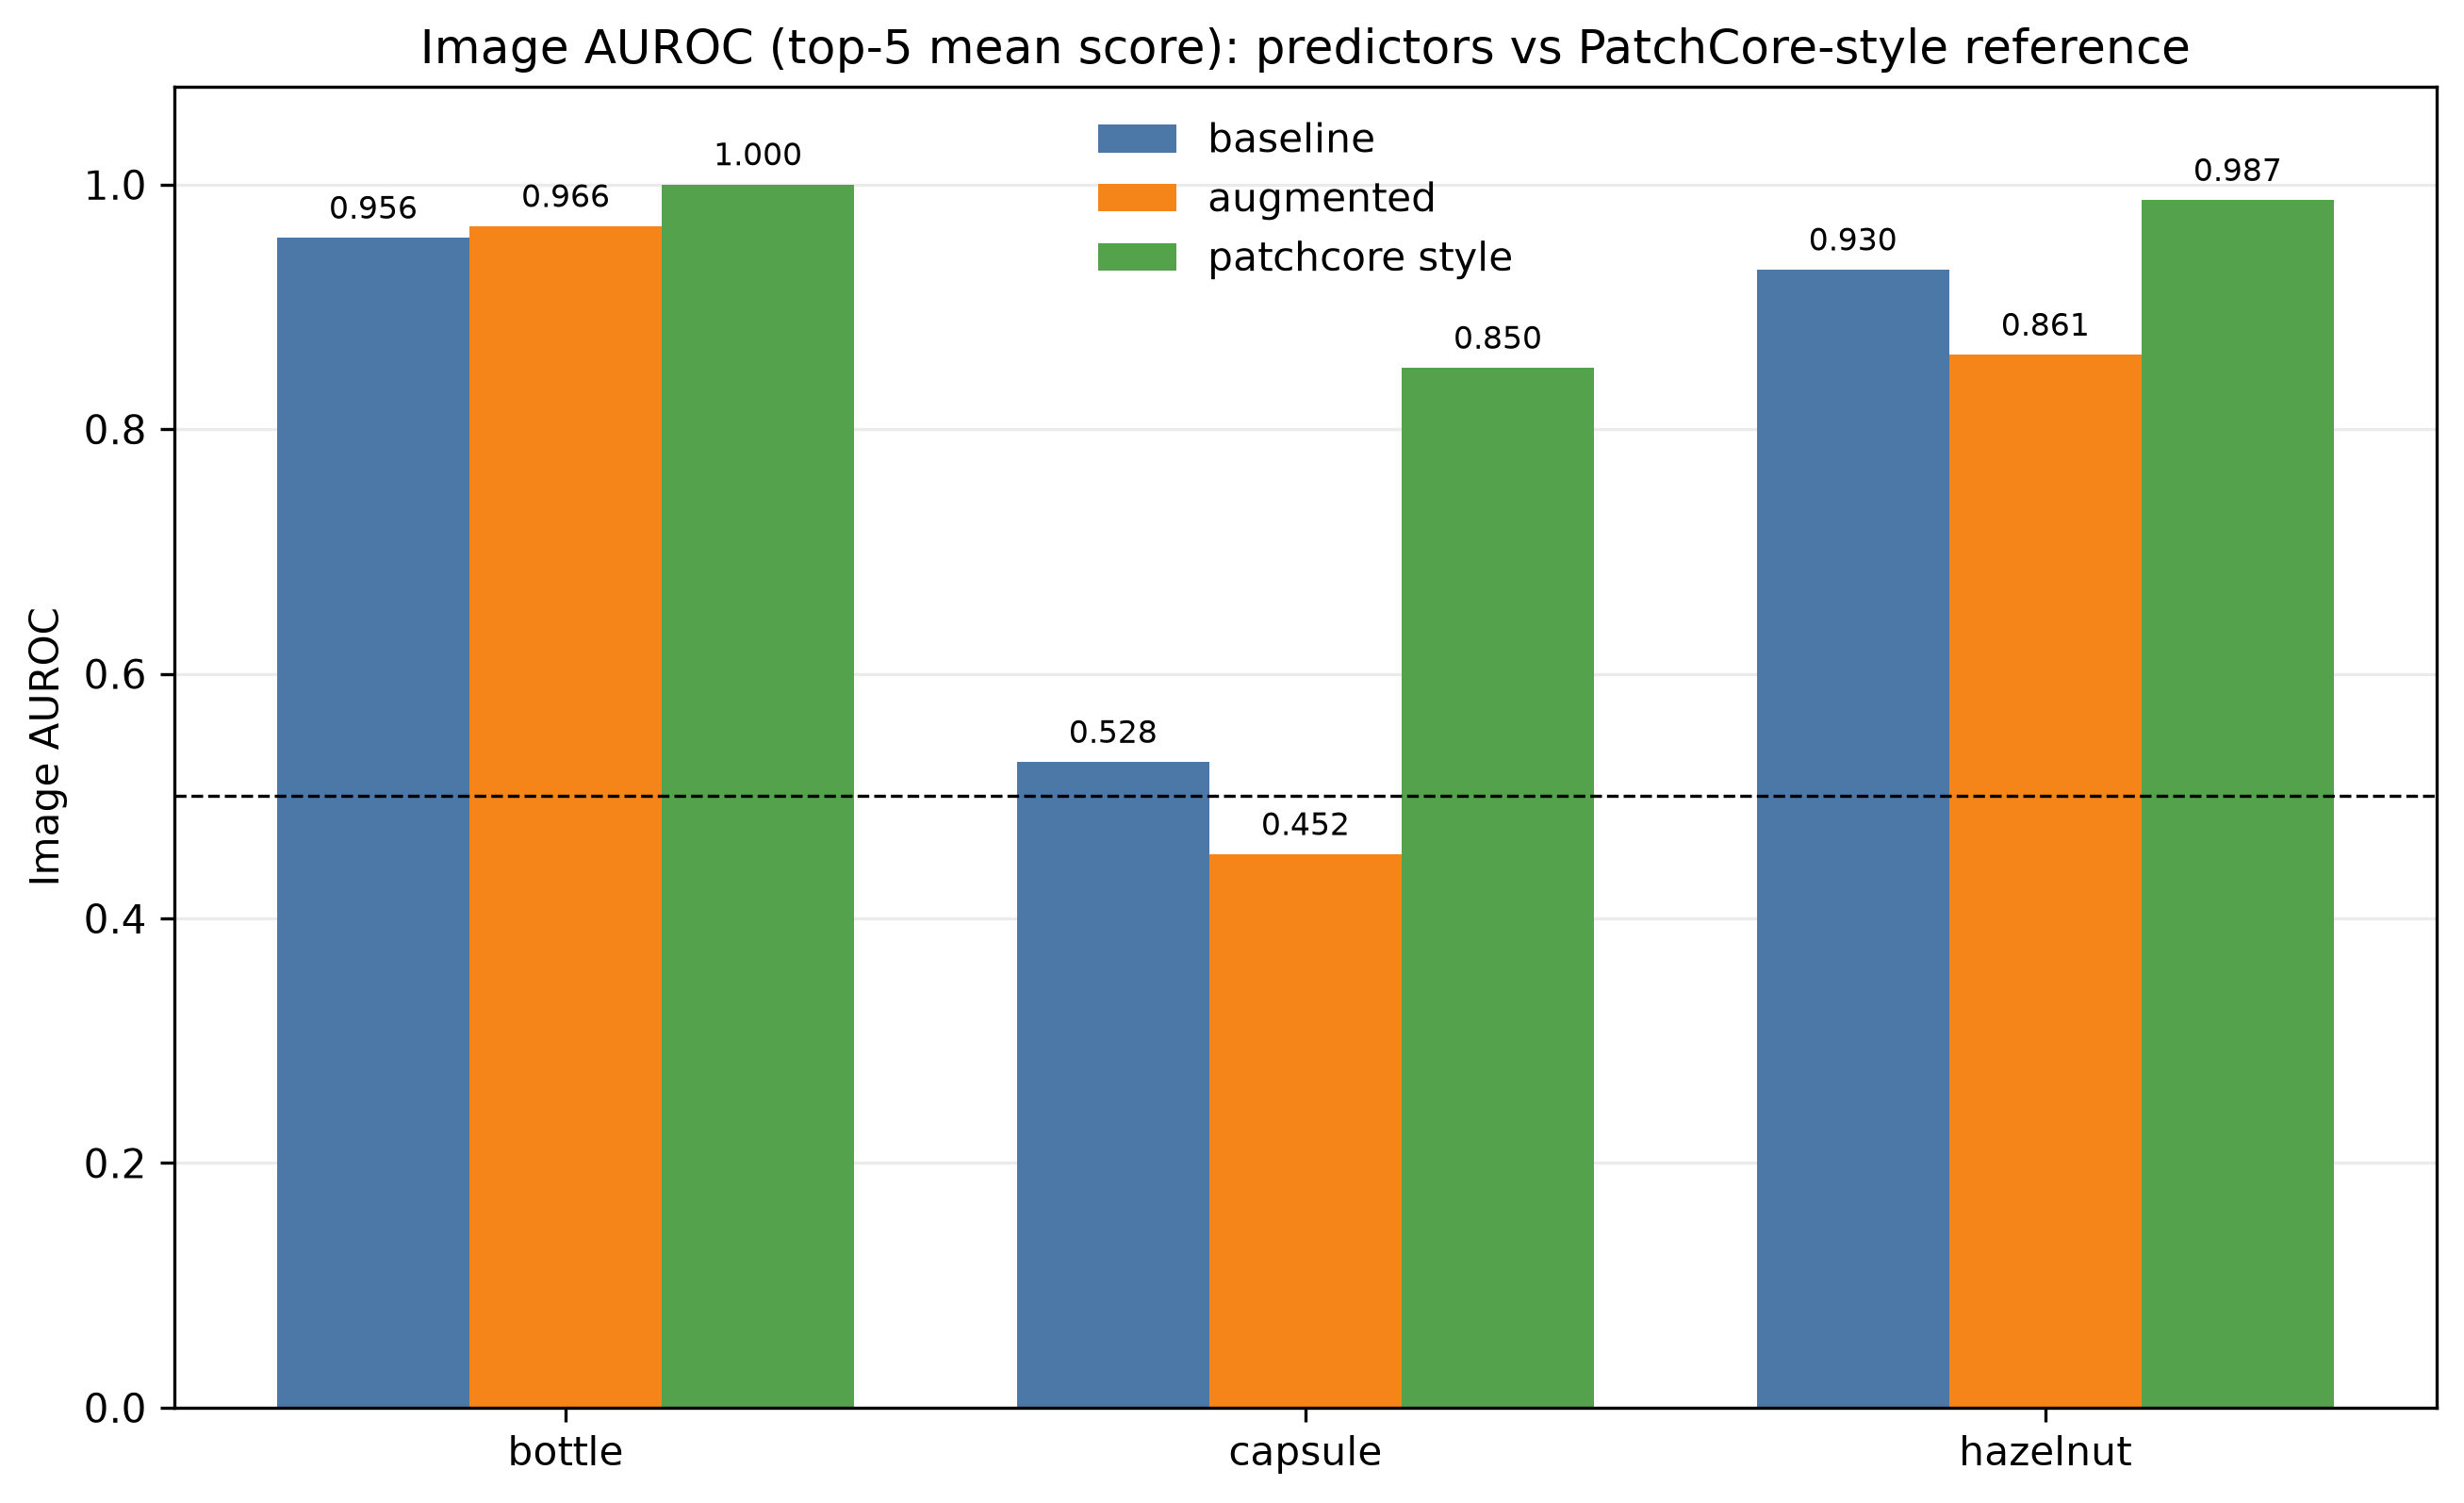
\includegraphics[width=\columnwidth]{figures/reference_comparison.png}
\caption{Image AUROC (top-5 mean score) of the baseline and augmented predictors versus the nearest-neighbour reference on the test split; values match Table~\ref{tab:main}.}
\label{fig:ref}
\end{figure}

\textbf{Against the reference.} The nearest-neighbour reference on identical latents beats the predictor-based detector in every category and every metric (mean pixel AUROC 0.956 vs 0.840, mean AUPRO 0.747 vs 0.480; Fig.~\ref{fig:ref}). The gap is largest for capsule and hazelnut. On these latents, directly comparing patches with the nominal memory bank was therefore a stronger signal than predicting masked latents from context. We return to this in Section~\ref{sec:disc}.

\textbf{Effect of augmentation.} Adding augmented nominal copies did \emph{not} help consistently. Image AUROC decreased in all three categories (mean $0.750\rightarrow0.678$), while pixel AUROC was essentially unchanged on average ($0.840$ vs $0.838$) and AUPRO changed by $-0.0002$ to $+0.023$. With 20--40 normal test images per category these differences are not conclusive, but they do not support augmentation as a remedy.

\subsection{Masking policy: accuracy versus cost}
Table~\ref{tab:modes} compares the masking policies using the same baseline predictors. Fixed, default-adaptive and dense masking produce nearly identical localisation: mean pixel AUROC is 0.840, 0.840 and 0.848 respectively, while dense masking needs $196/16=12.25\times$ as many predictor passes. Default-adaptive uses only 16.1 masks per image, a 91.8\,\% reduction from dense, and exceeds the planned target of at least 50\,\%. This saving, however, is almost entirely because the default gate ($\tau=0.5$) opens on only about one test image in a hundred for bottle and hazelnut and never for capsule (trigger rates 1.2\,\%, 0\,\% and 0.9\,\%), so the method behaves like the fixed coarse scheme. Raw discrepancies of nominal tokens on a validation set are far below 0.5 (Section~\ref{sec:calib}), which explains why the gate is inactive.

\begin{table}[t]
\caption{Pixel-level metrics and mean predictor passes per image for four masking policies (baseline predictors, test split). ``Cal.'' is the validation-calibrated gate with the 0.99 token quantile.}
\label{tab:modes}
\centering
\scriptsize
\setlength{\tabcolsep}{3pt}
\begin{tabular}{lccccccc}
\hline
 & \multicolumn{3}{c}{\textbf{Pixel AUROC}} & \multicolumn{3}{c}{\textbf{AUPRO}} & \textbf{Masks} \\
\textbf{Policy} & B & C & H & B & C & H & \textbf{(mean)} \\
\hline
Fixed (coarse only)  & .930 & .685 & .907 & .766 & .098 & .578 & 16.0 \\
Adaptive, $\tau{=}0.5$ & .930 & .685 & .907 & .766 & .098 & .577 & 16.1 \\
Adaptive, cal.\ $\tau$ & .926 & .700 & .923 & .732 & .103 & .566 & 34.7 \\
Dense (196 masks)    & .928 & .706 & .909 & .762 & .111 & .584 & 196 \\
\hline
\end{tabular}
\end{table}

\begin{figure*}[t]
\centering
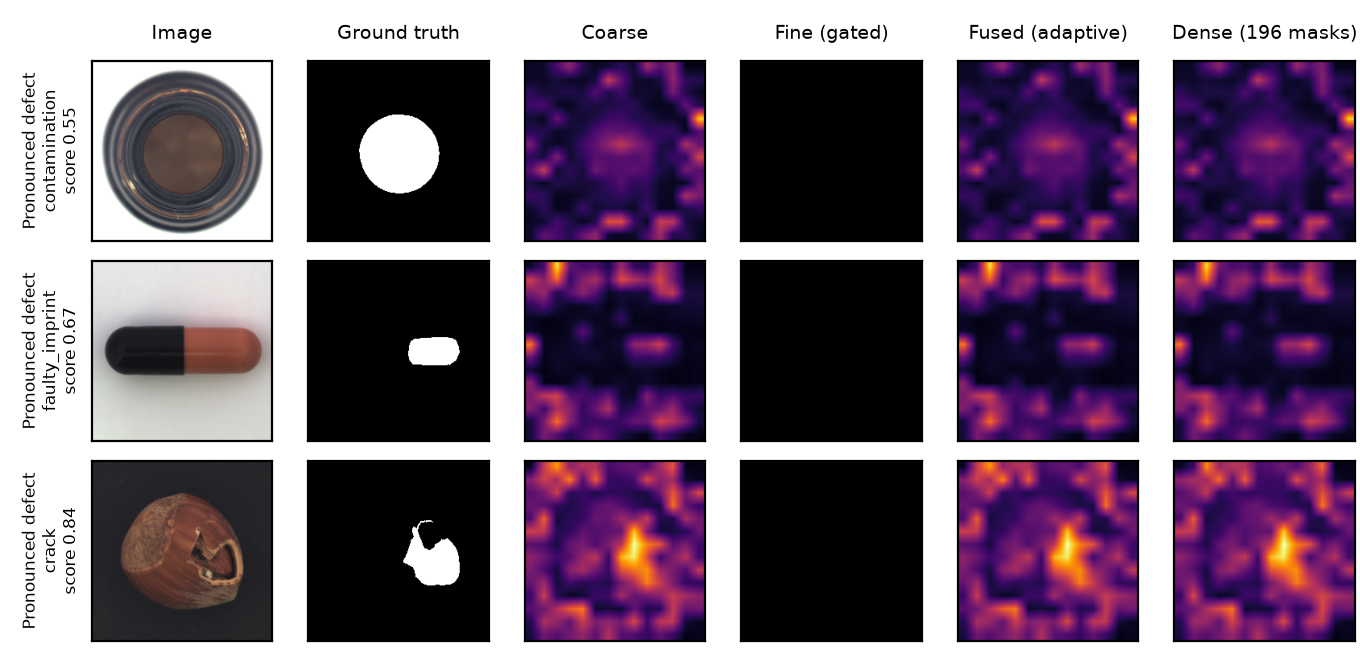
\includegraphics[width=0.92\textwidth]{figures/heatmaps_composite.png}
\caption{Raw cosine-discrepancy maps for one pronounced defect per category (top to bottom: bottle, capsule, hazelnut). Columns: image, ground truth, coarse map, gated fine map, fused adaptive map and the dense reference. The fine map is empty because the default gate never fires on these images. Colour scales are relative within each row.}
\label{fig:heat}
\end{figure*}

Fig.~\ref{fig:heat} shows qualitative maps. For hazelnut, the crack is clearly highlighted by both coarse and dense maps, and the fused adaptive map is visually indistinguishable from the dense one. For the bottle contamination, the discrepancy is spread diffusely over the interior and is weaker than the response at the image border, which hurts image-level ranking. For capsule, the faulty imprint is only weakly highlighted relative to responses elsewhere, consistent with chance-level image AUROC. Border patches often show high discrepancy even for nominal images, because they have less context to predict from.

\begin{figure*}[t]
\centering
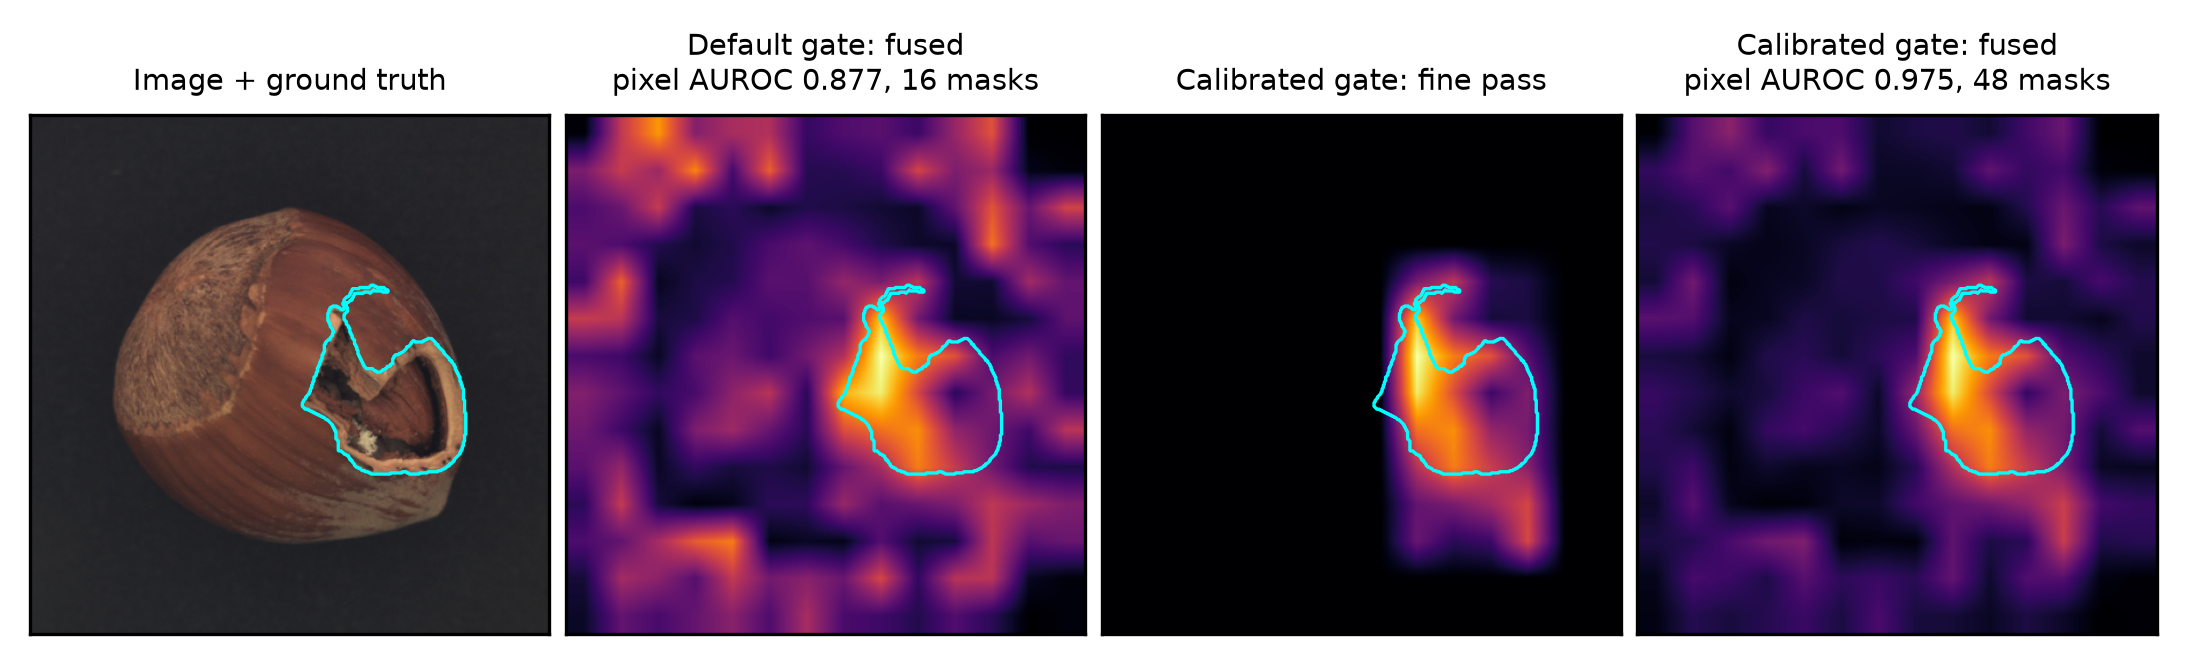
\includegraphics[width=0.95\textwidth]{figures/heatmap_hazelnut_calibrated.png}
\caption{Hazelnut crack with the default and the calibrated gate (baseline predictor). The cyan contour is the ground truth. With the calibrated gate ($\tau=0.350$) the fine pass fires on 32 tokens around the defect (48 masks in total instead of 16) and the fused map suppresses background clutter. Each panel is min-max normalised for display only; pixel AUROC is computed per image on the raw map. This is the one example where the calibrated gate helped clearly; see the text for the other two.}
\label{fig:hazcal}
\end{figure*}

Fig.~\ref{fig:hazcal} repeats the hazelnut crack with the calibrated gate. The fine pass now fires on 32 tokens around the defect, concentrates the response on the crack, and raises the per-image pixel AUROC from 0.877 to 0.975. We show this case because hazelnut is the category where the calibrated setting gave a gain whose bootstrap interval excludes zero and where mean pixel AUROC rose (0.907 to 0.923). It is the best case and not a typical one: for the bottle contamination the same gate \emph{lowered} per-image pixel AUROC from 0.784 to 0.736 (40 masks), and for the capsule imprint the fine pass never fired, so the map and the score (0.705) are unchanged. We therefore do not replace Fig.~\ref{fig:heat} with calibrated maps for the other categories.

\subsection{Latency and memory}
Table~\ref{tab:latency} and Fig.~\ref{fig:lat} give the cost on an 8~GB RTX 4060. The frozen ViT-g/16 dominates fixed and adaptive inference: it uses 3.94~GB of FP32 weights and 87.5~ms per image, and peak memory during scoring is 4.08~GB, so the whole pipeline fits an 8~GB card. Adaptive masking adds 8.9~ms over fixed masking at end-to-end level (133.8 vs 124.9~ms), while dense masking is $2.6\times$ slower than adaptive (349.8~ms). The nearest-neighbour reference scores a test image in 8.0~ms but stores a 198~MB bank of 36{,}848 patches (bottle), and its peak memory including the bank is 4.63~GB.

\begin{table}[t]
\caption{Latency and memory on an RTX 4060 (8~GB), FP32 encoder. Left: end-to-end (mean $\pm$ std over 40 images). Right: predictor-only scoring on cached latents, per category (bottle/capsule/hazelnut).}
\label{tab:latency}
\centering
\scriptsize
\setlength{\tabcolsep}{3pt}
\begin{tabular}{lccc}
\hline
\textbf{Policy} & \textbf{End-to-end (ms)} & \textbf{P95 (ms)} & \textbf{Scoring only B/C/H (ms)} \\
\hline
Encoder only (batch 1) & $87.5\pm5.4$  & 100.5 & -- \\
Fixed    & $124.9\pm3.5$  & 130.2 & 18.1 / 17.5 / 17.5 \\
Adaptive & $133.8\pm4.4$  & 141.3 & 30.4 / 20.6 / 21.1 \\
Dense    & $349.8\pm10.1$ & 367.9 & 214.4 / 216.7 / 238.1 \\
\hline
\multicolumn{4}{l}{Peak GPU memory: 4078~MB (all three policies); encoder weights 3939~MB.}
\end{tabular}
\end{table}

\begin{figure}[t]
\centering
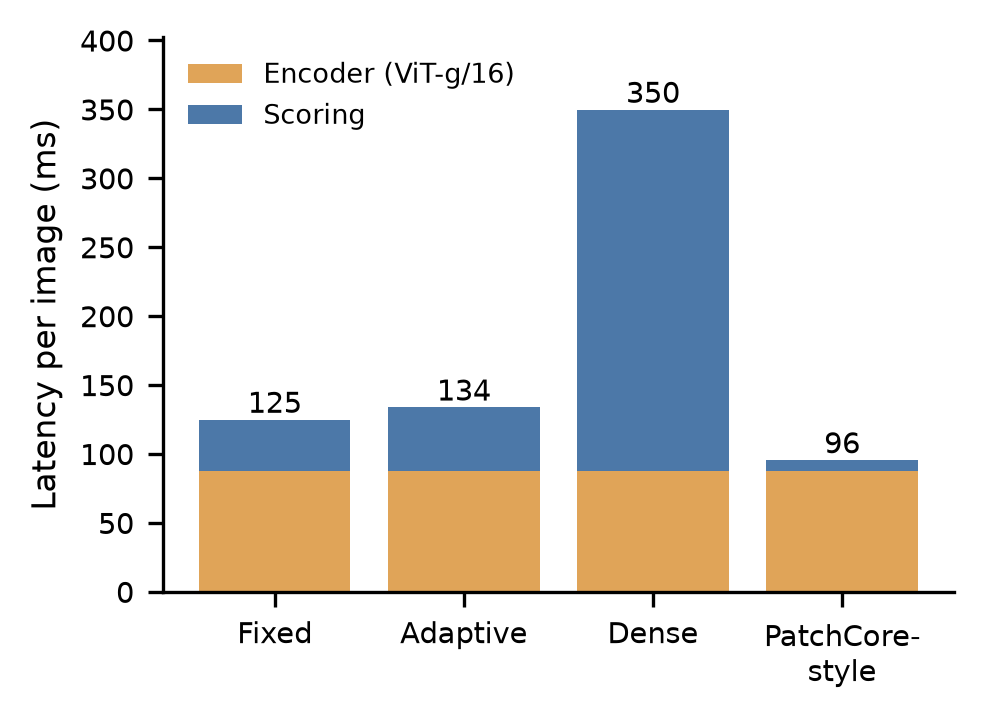
\includegraphics[width=0.8\columnwidth]{figures/latency_e2e.png}
\caption{End-to-end latency per image split into encoder and scoring time. The PatchCore-style bar adds the measured 8.0~ms bank search to the encoder time.}
\label{fig:lat}
\end{figure}

%==============================================================================
\section{Validation-Only Calibration of the Gate and Image Score}\label{sec:calib}
The default gate is inactive and the max-patch image score lets a single noisy patch decide an image. We test two inexpensive fixes that need no retraining, under a protocol that never uses test labels for selection: the primary setting (token quantile 0.99, top-5 mean, $\lambda=1$) was declared \emph{before} any test result was inspected, the gate threshold $\tau$ is set from nominal validation images only, and the other grid cells are reported as a sensitivity view and not as a selection.

\textbf{Gate calibration.} For each category, $\tau$ is the $q$-quantile of region scores pooled over all validation tokens, so that the fine pass fires on about $1-q$ of normal tokens. Table~\ref{tab:gate} shows that the default $\tau=0.5$ opens on 0\,\% of nominal validation images, whereas $q=0.99$ gives about 2 fine passes per normal image, triggering on 19--23\,\% of normal images. Calibrated thresholds are small ($\tau\approx0.16$--$0.35$) because the predictor reproduces nominal latents well.

\begin{table}[t]
\caption{Gate calibration on nominal validation images. For each category: $\tau$ / fine windows per nominal image / \% nominal images triggering a fine pass.}
\label{tab:gate}
\centering
\scriptsize
\setlength{\tabcolsep}{3pt}
\begin{tabular}{lccc}
\hline
\textbf{Gate} & \textbf{Bottle} & \textbf{Capsule} & \textbf{Hazelnut} \\
\hline
Default        & .500 / 0.0 / 0   & .500 / 0.0 / 0    & .500 / 0.0 / 0 \\
$q=0.9$        & .098 / 19.8 / 86 & .207 / 19.6 / 91 & .279 / 19.7 / 92 \\
$q=0.95$       & .123 / 9.9 / 62  & .225 / 9.8 / 68  & .307 / 9.8 / 74 \\
$q=0.99$       & .158 / 2.3 / 19  & .264 / 2.2 / 23  & .350 / 2.1 / 23 \\
$q=0.995$      & .184 / 1.1 / 14  & .282 / 1.1 / 14  & .368 / 1.0 / 13 \\
\hline
\end{tabular}
\end{table}

\textbf{Image score and statistical evidence.} Fig.~\ref{fig:k} shows image AUROC as a function of $k$ for the default and calibrated gates. Because the test sets contain only 20--40 normal images, we resample test images (good and anomalous separately, 1000 paired bootstrap draws) and report 95\,\% intervals for the change in image AUROC relative to the original pipeline (default gate, max score) in Table~\ref{tab:boot}.

\begin{figure*}[t]
\centering
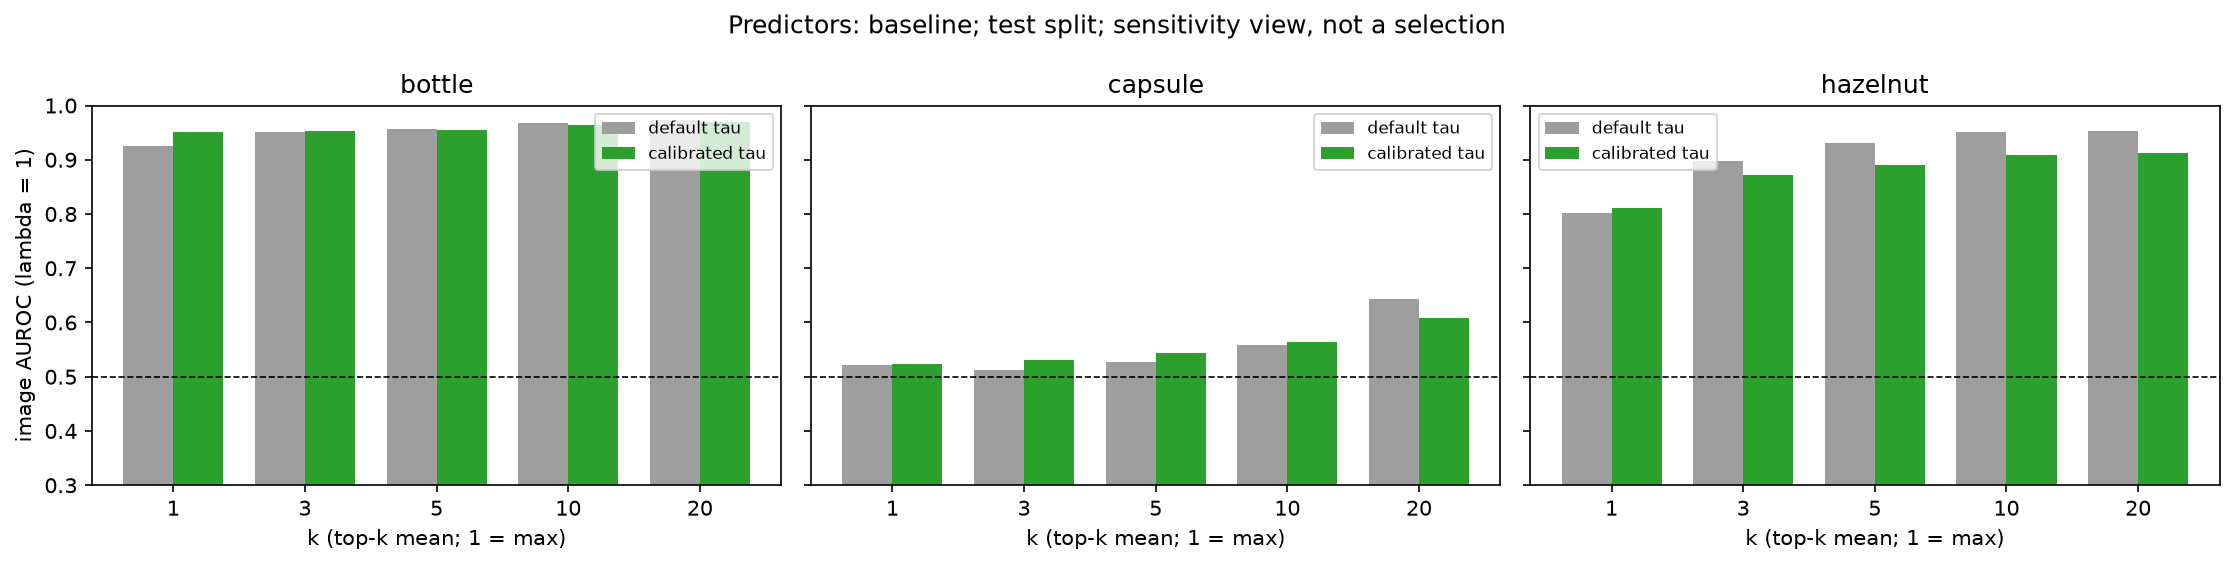
\includegraphics[width=0.92\textwidth]{figures/image_auroc_vs_k.png}
\caption{Image AUROC versus $k$ of the top-$k$ mean score ($k=1$ is the max score) with $\lambda=1$, for the default and calibrated gates (baseline predictors, test split). The dashed line is chance. This is a sensitivity view, not a selection.}
\label{fig:k}
\end{figure*}

\begin{table}[t]
\caption{Paired-bootstrap change in image AUROC versus the original pipeline (default gate, max score), with 95\,\% interval. Asterisk: interval excludes zero.}
\label{tab:boot}
\centering
\scriptsize
\setlength{\tabcolsep}{2.5pt}
\begin{tabular}{lccc}
\hline
\textbf{Category} & \textbf{Gate only} & \textbf{Top-5 only} & \textbf{Both (primary)} \\
\hline
Bottle   & +.026 [$-$.037, +.097] & +.032 [$-$.005, +.078] & +.030 [$-$.026, +.097] \\
Capsule  & +.001 [$-$.114, +.107] & +.006 [$-$.126, +.153] & +.022 [$-$.128, +.180] \\
Hazelnut & +.009 [$-$.055, +.069] & +.128 [+.068, +.198]\textsuperscript{*} & +.088 [+.006, +.171]\textsuperscript{*} \\
\hline
\end{tabular}
\end{table}

The only statistically supported improvement is the top-5 mean score on hazelnut (and the combined setting there). Everywhere else the interval contains zero, so the data support neither an improvement nor a harm. The calibrated gate has a cost: the mean masks per image rises from 16.1 to 34.7 (an 82\,\% reduction from dense instead of 92\,\%) and, for bottle and hazelnut, AUPRO is lower than with the default gate (Table~\ref{tab:modes}). Pixel AUROC improves modestly for capsule and hazelnut (+.015 and +.017).

\textbf{Decision thresholds.} For deployment a decision threshold is calibrated on validation scores to a 5\,\% target false-positive rate. On the test set, the primary setting yields test false-positive and true-positive rates of 0.00/0.71 for bottle, 0.17/0.19 for capsule and 0.025/0.20 for hazelnut, versus 0.00/0.49, 0.22/0.14 and 0.025/0.11 for the original setting. With only 21--39 validation images the 5\,\% target allows a single exceedance, so these thresholds are rough; capsule's false-positive rate (0.17--0.22) is well above the target and shows that the threshold does not transfer there.

%==============================================================================
\section{Validation-Selected Improvements}\label{sec:improve}
The calibration of Section~\ref{sec:calib} used only nominal validation images, which contain no defects, so nothing could be chosen for \emph{detection} quality. This section adds a labelled validation set and uses it to choose the scoring settings and the encoder layer without reading the test split.

\textbf{Synthetic-defect validation set.} For every nominal validation image we generate four defects with a fixed seed, alternating CutPaste scars \cite{li2021cutpaste} (a jittered, rotated patch cut from elsewhere on the object) and DRAEM-style Perlin-noise texture blends \cite{zavrtanik2021draem}. Defects stay on the object and cover 0.3--4\,\% of the image; textures come from nominal training images. This gives 84, 88 and 156 synthetic images for bottle, capsule and hazelnut with exact masks, so image AUROC, pixel AUROC and AUPRO can be measured. Official test images are never read.

\textbf{Selection protocol (declared before any result was seen).} Statistics that are fitted (per-position z-score, Mahalanobis covariance, gate quantiles) are cross-fitted over three folds of the clean validation images, so no validation image is used both for fitting and for evaluation. Settings are chosen greedily in a fixed order (score family, smoothing $\sigma$, image-score $k$, fusion $\lambda$, gate $\tau$) with one criterion, the mean over categories of the average of image AUROC, pixel AUROC and AUPRO, and one global choice for all categories. Options within 0.005 of the best are treated as tied and the earlier (simpler) option wins. For the final-layer predictor this selected a per-token-position z-score of the patch score (each of the 196 positions normalised with the mean and standard deviation of nominal validation scores), $\sigma{=}0$, $k{=}3$, $\lambda{=}1$ and the default gate. After the selection was saved, the proxy's ranking of eight scoring variants agreed with the test split (mean Spearman 0.74 for image AUROC with the max score, 0.86 with top-5, 0.84 for pixel AUROC, 0.94 for AUPRO) but only weakly for capsule's max-score image AUROC (0.42).

\textbf{Encoder layer.} Final-layer tokens are semantic and spatially diffuse, whereas nearest-neighbour methods such as PatchCore use mid-level features. We cached tokens (parameter-free per-token layer norm) from blocks 8, 12, \dots, 40 of the frozen encoder and scored the nearest-neighbour reference on the synthetic set. Mid layers were best (criterion 0.987 for layers 24 and 28, 0.986 for layer 32, 0.969 for the final cached latents; block 40 before the final norm reproduced the final latents, which checks the pipeline). The declared rule selected layer 32; layers 24 and 28 are within the tie margin. We then trained predictors on layer-32 tokens with exactly the baseline recipe (architecture, optimiser, masks, seed), so only the input tokens differ.

\textbf{Results.} Table~\ref{tab:improved} and Table~\ref{tab:boot2} report the official test split. Position z-scoring alone (final layer) raises mean pixel AUROC from 0.840 to 0.941 and mean AUPRO from 0.480 to 0.717. Moving the predictor to layer 32 on top of it raises capsule image AUROC (top-3) from 0.672 to 0.767 (+0.095, interval [+0.038, +0.150]) and hazelnut from 0.939 to 0.993 (+0.054, [+0.017, +0.101]); bottle is at the ceiling (+0.002, inconclusive). The combination improves image AUROC over the original pipeline in all three categories (bottle +0.075, capsule +0.246, hazelnut +0.191; all intervals exclude zero) with the same 16.0--16.6 masks per image and a scorer latency of about 22 ms per image in the same measurement run. Without the z-score, layer 32 alone already helps hazelnut significantly and capsule only at the top-3 score, so the two changes are complementary. Mean pixel AUROC reaches 0.962 and mean AUPRO 0.813. The nearest-neighbour reference on layer-32 tokens remains stronger (mean image AUROC 0.97, AUPRO 0.88), so the gap to a memory-bank method is reduced, not closed, and capsule image AUROC (0.77 against 0.91) is still the weakest result.

\begin{table*}[t]
\caption{Test results after the validation-selected changes (official test split, one scoring pass per row). All layer-32 rows use the same predictor architecture, training recipe and masks as the baseline; only the cached tokens change. Image AUROC is given for the max score and for the mean of the top-3 token scores. The z-score settings (position z-score, $k{=}3$) were chosen on synthetic validation defects for the final-layer predictor and carried over unchanged; layer 32 was chosen on the same synthetic data. \textsuperscript{a}Re-selected on layer-32 synthetic validation data and scored once on test; its score is the max (top-3 shown for comparison only). \textsuperscript{b}Nearest-neighbour reference on layer-32 tokens (full memory bank), context only.}
\label{tab:improved}
\centering
\footnotesize
\begin{tabular}{llccccc}
\hline
\textbf{Category} & \textbf{Method} & \textbf{Img AUROC (max)} & \textbf{Img AUROC (top-3)} & \textbf{Pixel AUROC} & \textbf{AUPRO} & \textbf{Masks/img} \\
\hline
\multirow{6}{*}{Bottle}
 & Original baseline (final layer, $1-\cos$) & 0.925 & 0.952 & 0.930 & 0.766 & 16.2 \\
 & + position z-score (final layer) & 0.993 & 0.998 & 0.952 & 0.831 & 16.2 \\
 & Layer 32, $1-\cos$ & 0.959 & 0.975 & 0.979 & 0.904 & 16.2 \\
 & \textbf{Layer 32 + position z-score} & 0.994 & 0.999 & 0.966 & 0.871 & 16.2 \\
 & Layer 32 + Mahalanobis $d{=}128$\textsuperscript{a} & 0.991 & 0.998 & 0.983 & 0.928 & 16.2 \\
 & kNN reference, layer 32\textsuperscript{b} & 1.000 & 1.000 & 0.987 & 0.937 & -- \\
\hline
\multirow{6}{*}{Capsule}
 & Original baseline (final layer, $1-\cos$) & 0.522 & 0.512 & 0.684 & 0.098 & 16.0 \\
 & + position z-score (final layer) & 0.622 & 0.672 & 0.901 & 0.508 & 16.0 \\
 & Layer 32, $1-\cos$ & 0.543 & 0.660 & 0.836 & 0.309 & 16.0 \\
 & \textbf{Layer 32 + position z-score} & 0.721 & 0.767 & 0.931 & 0.666 & 16.0 \\
 & Layer 32 + Mahalanobis $d{=}128$\textsuperscript{a} & 0.600 & 0.647 & 0.956 & 0.720 & 16.0 \\
 & kNN reference, layer 32\textsuperscript{b} & 0.909 & 0.909 & 0.962 & 0.771 & -- \\
\hline
\multirow{6}{*}{Hazelnut}
 & Original baseline (final layer, $1-\cos$) & 0.802 & 0.897 & 0.907 & 0.577 & 16.1 \\
 & + position z-score (final layer) & 0.864 & 0.939 & 0.969 & 0.812 & 16.1 \\
 & Layer 32, $1-\cos$ & 0.946 & 0.989 & 0.986 & 0.877 & 16.6 \\
 & \textbf{Layer 32 + position z-score} & 0.981 & 0.993 & 0.989 & 0.901 & 16.6 \\
 & Layer 32 + Mahalanobis $d{=}128$\textsuperscript{a} & 0.960 & 0.969 & 0.987 & 0.894 & 16.6 \\
 & kNN reference, layer 32\textsuperscript{b} & 0.999 & 1.000 & 0.995 & 0.941 & -- \\
\hline
\multirow{6}{*}{Mean}
 & Original baseline (final layer, $1-\cos$) & 0.750 & 0.787 & 0.840 & 0.480 & 16.1 \\
 & + position z-score (final layer) & 0.826 & 0.870 & 0.941 & 0.717 & 16.1 \\
 & Layer 32, $1-\cos$ & 0.816 & 0.875 & 0.934 & 0.697 & 16.3 \\
 & \textbf{Layer 32 + position z-score} & 0.899 & 0.920 & 0.962 & 0.813 & 16.3 \\
 & Layer 32 + Mahalanobis $d{=}128$\textsuperscript{a} & 0.850 & 0.871 & 0.975 & 0.847 & 16.3 \\
 & kNN reference, layer 32\textsuperscript{b} & 0.969 & 0.970 & 0.981 & 0.883 & -- \\
\hline
\end{tabular}
\end{table*}

\begin{table*}[t]
\caption{Paired-bootstrap change in image AUROC on the test split (1,000 resamples, same resamples for all comparisons within a category, 95\,\% interval). Asterisk: interval excludes zero. Rows 1--4 use configurations fixed before their test evaluation; rows 5--7 evaluate the layer-32 re-selection (Mahalanobis).}
\label{tab:boot2}
\centering
\scriptsize
\setlength{\tabcolsep}{3pt}
\begin{tabular}{lccc}
\hline
\textbf{Comparison (new vs reference)} & \textbf{Bottle} & \textbf{Capsule} & \textbf{Hazelnut} \\
\hline
Final layer + z-score (top-3) vs original (max) & +0.073 [+0.019, +0.152]\textsuperscript{*} & +0.150 [$-$0.045, +0.356] & +0.137 [+0.054, +0.226]\textsuperscript{*} \\
Layer 32 + z-score (top-3) vs original (max) & +0.075 [+0.021, +0.153]\textsuperscript{*} & +0.246 [+0.049, +0.457]\textsuperscript{*} & +0.191 [+0.107, +0.284]\textsuperscript{*} \\
Layer 32 + z-score vs final layer + z-score (top-3) & +0.002 [+0.000, +0.007] & +0.095 [+0.038, +0.150]\textsuperscript{*} & +0.054 [+0.017, +0.101]\textsuperscript{*} \\
Layer 32, $1-\cos$ vs original (max) & +0.034 [$-$0.024, +0.110] & +0.021 [$-$0.075, +0.114] & +0.144 [+0.061, +0.239]\textsuperscript{*} \\
Layer 32 Mahalanobis vs layer 32 $1-\cos$ (max) & +0.033 [+0.004, +0.078]\textsuperscript{*} & +0.057 [$-$0.123, +0.259] & +0.013 [$-$0.031, +0.068] \\
Layer 32 Mahalanobis (max) vs layer 32 z-score (top-3) & $-$0.008 [$-$0.029, +0.002] & $-$0.167 [$-$0.282, $-$0.057]\textsuperscript{*} & $-$0.034 [$-$0.067, $-$0.007]\textsuperscript{*} \\
Layer 32 Mahalanobis (max) vs original (max) & +0.067 [+0.012, +0.144]\textsuperscript{*} & +0.079 [$-$0.134, +0.303] & +0.157 [+0.076, +0.254]\textsuperscript{*} \\
\hline
\end{tabular}
\end{table*}


\textbf{Re-selection for layer 32 (a negative result).} Because the settings were chosen for the final-layer predictor, we repeated the same selection protocol on the layer-32 predictors and synthetic data, again without touching the test split. It chose a Mahalanobis residual score (PCA to 128 components, fitted on nominal validation residuals) with the max score; it was then scored once on the test split. Against raw cosine on the same layer-32 predictor it improves bottle (+0.033, [+0.004, +0.078]) and is inconclusive for capsule and hazelnut, and its pixel AUROC and AUPRO are higher (mean 0.976 and 0.847, point estimates). At image level, however, it is \emph{worse} than the z-score configuration reported above (capsule $-0.167$, [$-0.282$, $-0.057$]; hazelnut $-0.034$, [$-0.067$, $-0.007$]; Table~\ref{tab:boot2}). We therefore report the configuration that was fixed before this re-selection as the headline and the Mahalanobis result as a negative finding on how well synthetic validation transfers: the Mahalanobis dimension is a strongly sensitive setting ($d{=}32/64/128$ score 0.87/0.92/0.96 on the criterion, and 128 is the largest value in the grid) and the synthetic criterion is close to its ceiling.

\textbf{Pretrained predictor and leakage.} Our masking acts on latents after full-image encoding, so context tokens may already contain the defect. As a first test we ran Meta's pretrained I-JEPA context encoder and predictor on the visible tokens only (zero-shot, ImageNet-22k). It did not beat our predictor (image AUROC with the z-score: bottle 0.986 against 0.998, capsule 0.647 against 0.672, hazelnut 0.809 against 0.939, the last significantly lower), and costs about 980\,ms per image against 23\,ms. Leakage is therefore not supported as the main limit, but the test is confounded (predictor size and training data also differ); a decisive test would retrain our predictor on input-masked context latents.

\textbf{Limitations of this section.} Each predictor is a single training run per category; the synthetic defects are a stand-in for MVTec defects and no proxy-versus-test check exists for layer 32; capsule intervals are wide (132 test images); layers 24 and 28 were not trained as predictors; and the headline top-3 score is compared with the original max score in two of the rows (the same-score comparison is the third row of Table~\ref{tab:boot2}).

%==============================================================================
\section{Discussion}\label{sec:disc}
\textbf{What worked.} The pipeline is decoder-free, fits in 8~GB, and runs end to end in 134~ms. Latent prediction yields a usable localisation signal for categories with regular structure (bottle pixel AUROC 0.93; hazelnut 0.91), and the coarse scheme gets nearly the same localisation as dense masking at 8\,\% of the predictor passes.

\textbf{What did not.} (i) The adaptive refinement did not add accuracy: with the default gate it never fires, and with a calibrated gate fine passes help clearly on some images (the hazelnut crack in Fig.~\ref{fig:hazcal}) but not consistently: mean AUPRO falls and bottle gets worse (Table~\ref{tab:modes}). On this pilot we therefore cannot claim that adaptivity reliably improves over coarse masking. Its value here is limited to avoiding dense masking, which fixed masking also achieves. (ii) Capsule image AUROC stays between 0.40 and 0.52 for the max score and reaches at most 0.64 at $k=20$ (Fig.~\ref{fig:k}), which suggests that the predictor does not separate its defects (small imprint and surface faults) from natural variability; a $2\times2$ coarse-window checkpoint for capsule did not beat the baseline either. These statements concern the original pipeline; Section~\ref{sec:improve} shows that capsule improves with mid-level tokens and score normalisation. (iii) The nearest-neighbour reference on identical latents is clearly better, so the detection signal is present in the frozen latents but is not extracted as well by context prediction. Section~\ref{sec:improve} tests part of this: a large share of the gap comes from using final-layer tokens and unnormalised cosine scores, since layer-32 tokens and a per-position z-score recover much of it. Whether the predictors underfit on only 188--352 nominal images was not tested.

\textbf{Threats to validity.}
\begin{itemize}
\item \emph{Scope.} Only 3 of the 15 MVTec AD categories were evaluated; the other 12, MVTec AD 2 and a valid MAE baseline are outstanding. These results are pilot evidence and not a benchmark claim.
\item \emph{Sample size.} Validation sets have 21--39 images and test sets 20--40 normal images, so AUROC differences of a few points are within noise; we used a single seed and no variance across training runs.
\item \emph{Possible context leakage.} Masking is applied to the latent grid after full-image encoding, so context tokens were computed with attention over the masked region. A zero-shot test with Meta's pretrained predictor and input masking did not help, but it is confounded; retraining on input-masked latents was not done.
\item \emph{Synthetic validation.} Settings and the layer were chosen on CutPaste and Perlin defects, which are not MVTec defects. The proxy ranked scoring variants like the test split on average but weakly for capsule, and a re-selection for layer 32 did not transfer to image-level test performance.
\item \emph{Reference baseline.} The nearest-neighbour row uses final-layer latents and a full memory bank and is not the original PatchCore with mid-level features and coreset subsampling. It is a context row and not a reproduction of published PatchCore numbers.
\item \emph{Latency scope.} Cached-latent scoring excludes encoding, and the single-run latencies were not repeated across sessions (adaptive bottle scoring, for example, is 30~ms in one run and 25~ms in another).
\item \emph{Validation reuse.} The same nominal validation set is used for early stopping and for threshold calibration, which makes the false-positive control slightly optimistic.
\end{itemize}

\textbf{Future work.} The immediate steps are: the remaining 12 categories and multiple seeds; evaluating smaller coarse windows for capsule; multi-seed runs with a validation-locked configuration, and a validation-only study of mask block size, augmentation, training length and layers 24 and 28 as predictors; a faithful PatchCore and MAE baseline under the same protocol; retraining on input-masked latents to measure leakage, and higher input resolution or an object crop for capsule.

%==============================================================================
\section{Conclusion}
We presented I-JEPA-AD, a decoder-free anomaly detector that predicts masked regions in the latent space of a frozen I-JEPA ViT-g/16 and refines suspicious regions with a gated fine pass. On a three-category MVTec AD pilot it localises defects with mean pixel AUROC 0.84 using 16 predictor passes per image and 134~ms end-to-end latency on an 8~GB GPU, a $2.6\times$ speed-up over dense masking at equal localisation quality. A gate calibrated on validation data lifts mean image AUROC from 0.750 to 0.796 and helps visibly on hazelnut, but the adaptive gate did not give a consistent accuracy benefit across categories (mean AUPRO fell, bottle got worse), capsule defects were not detected by the original pipeline, and a nearest-neighbour baseline on the same latents is stronger. Choosing the encoder layer and the score normalisation on synthetic defects, without the test split, then gives large gains: with the same 16 masks per image, mean pixel AUROC rises to 0.96, mean AUPRO from 0.48 to 0.81 and mean image AUROC (top-3) to 0.92, with paired-bootstrap improvements over the original pipeline in every category and capsule rising from near chance to 0.77. A nearest-neighbour reference on the same tokens remains stronger at image level, and a layer-32 re-selection (Mahalanobis) did not transfer to the test split at image level. Validation-only selection with bootstrap intervals makes these conclusions auditable. Whether coarse-to-fine latent prediction can match embedding-based methods remains open and requires the full benchmark, stronger predictors and fair baselines.

%==============================================================================
\section*{Reproducibility}
Code, configurations, result tables and all figures are in the project repository. Reported results use the official checkpoint \texttt{IN22K-vit.g.16-600e} (SHA-256 beginning \texttt{a373c7b1}) and the official I-JEPA source at commit \texttt{52c1ae9}. Predictor checkpoints record the seed, training configuration, mask strategy and the hashes of their training and validation images. Tuning decisions were declared before the test set was scored and are recorded in the calibration summary. The synthetic validation set is fixed by seed and fingerprint (\texttt{46c947cb99e1faf4}), selections are saved as JSON records with the data and cache provenance (layer-32 tokens carry a derived checkpoint identity so they cannot be mixed with final-layer ones), and the tables of Section~\ref{sec:improve} are generated from the saved result files by \texttt{paper/make\_improvement\_tables.py}.

\begin{thebibliography}{00}
\bibitem{assran2023ijepa} M. Assran, Q. Duval, I. Misra, P. Bojanowski, P. Vincent, M. Rabbat, Y. LeCun, and N. Ballas, ``Self-supervised learning from images with a joint-embedding predictive architecture,'' in \emph{Proc. IEEE/CVF Conf. Comput. Vis. Pattern Recognit. (CVPR)}, 2023, pp. 15619--15629.
\bibitem{he2022mae} K. He, X. Chen, S. Xie, Y. Li, P. Doll\'ar, and R. Girshick, ``Masked autoencoders are scalable vision learners,'' in \emph{Proc. IEEE/CVF Conf. Comput. Vis. Pattern Recognit. (CVPR)}, 2022, pp. 16000--16009.
\bibitem{bergmann2019mvtec} P. Bergmann, M. Fauser, D. Sattlegger, and C. Steger, ``MVTec AD --- a comprehensive real-world dataset for unsupervised anomaly detection,'' in \emph{Proc. IEEE/CVF Conf. Comput. Vis. Pattern Recognit. (CVPR)}, 2019, pp. 9592--9600.
\bibitem{bergmann2021mvtec} P. Bergmann, K. Batzner, M. Fauser, D. Sattlegger, and C. Steger, ``The MVTec anomaly detection dataset: A comprehensive real-world dataset for unsupervised anomaly detection,'' \emph{Int. J. Comput. Vis.}, vol. 129, no. 4, pp. 1038--1059, 2021.
\bibitem{roth2022patchcore} K. Roth, L. Pemula, J. Zepeda, B. Sch\"olkopf, T. Brox, and P. Gehler, ``Towards total recall in industrial anomaly detection,'' in \emph{Proc. IEEE/CVF Conf. Comput. Vis. Pattern Recognit. (CVPR)}, 2022, pp. 14318--14328.
\bibitem{defard2021padim} T. Defard, A. Setkov, A. Loesch, and R. Audigier, ``PaDiM: A patch distribution modeling framework for anomaly detection and localization,'' in \emph{Int. Conf. Pattern Recognit. (ICPR) Workshops}, 2021, pp. 475--489.
\bibitem{zavrtanik2021draem} V. Zavrtanik, M. Kristan, and D. Sko\v{c}aj, ``DRAEM --- a discriminatively trained reconstruction embedding for surface anomaly detection,'' in \emph{Proc. IEEE/CVF Int. Conf. Comput. Vis. (ICCV)}, 2021, pp. 8330--8339.
\bibitem{zavrtanik2021inpainting} V. Zavrtanik, M. Kristan, and D. Sko\v{c}aj, ``Reconstruction by inpainting for visual anomaly detection,'' \emph{Pattern Recognit.}, vol. 112, art. 107706, 2021.
\bibitem{li2021cutpaste} C.-L. Li, K. Sohn, J. Yoon, and T. Pfister, ``CutPaste: Self-supervised learning for anomaly detection and localization,'' in \emph{Proc. IEEE/CVF Conf. Comput. Vis. Pattern Recognit. (CVPR)}, 2021, pp. 9664--9674.
\bibitem{batzner2024efficientad} K. Batzner, L. Heckler, and R. K\"onig, ``EfficientAD: Accurate visual anomaly detection at millisecond-level latencies,'' in \emph{Proc. IEEE/CVF Winter Conf. Appl. Comput. Vis. (WACV)}, 2024, pp. 128--138.
\bibitem{akcay2022anomalib} S. Akcay, D. Ameln, A. Vaidya, B. Lakshmanan, N. Ahuja, and U. Genc, ``Anomalib: A deep learning library for anomaly detection,'' in \emph{Proc. IEEE Int. Conf. Image Process. (ICIP)}, 2022, pp. 1706--1710.
\bibitem{lecun2022path} Y. LeCun, ``A path towards autonomous machine intelligence, version 0.9.2,'' OpenReview, 2022.
\end{thebibliography}

\end{document}
